\documentclass[12pt,a4paper]{article}

% ------------------------------------------------------------
% Packages and formatting required by the assignment
% ------------------------------------------------------------
\usepackage[utf8]{inputenc}
\usepackage[margin=1in, headheight=15pt]{geometry}
\usepackage{mathptmx}
\usepackage{amsmath}
\usepackage{amssymb}
\usepackage{booktabs}
\usepackage{array}
\usepackage{tabularx}
\usepackage{longtable}
\usepackage{enumitem}
\usepackage{float}
\usepackage{graphicx}
\usepackage{xcolor}
\usepackage{tikz}
\usepackage{caption}
\usepackage{listings}
\usepackage{hyperref}
\usepackage{fancyhdr}
\usepackage{setspace}
\usepackage[nobottomtitles*]{titlesec}

\usetikzlibrary{arrows.meta, positioning}

\hypersetup{
    colorlinks=true,
    linkcolor=black,
    citecolor=black,
    urlcolor=black
}

\titleformat{\section}{\Large\bfseries}{}{0em}{}
\titleformat{\subsection}{\large\bfseries}{}{0em}{}
\titleformat{\subsubsection}{\normalsize\bfseries}{}{0em}{}
\setlength{\parindent}{0pt}
\setlength{\parskip}{0.55em}
\onehalfspacing
\sloppy

\lstset{
    basicstyle=\ttfamily\small,
    breaklines=true,
    frame=single,
    backgroundcolor=\color{gray!10},
    numbers=left,
    numberstyle=\tiny\color{gray},
    numbersep=8pt,
    showstringspaces=false,
    tabsize=4,
    captionpos=b
}

\pagestyle{fancy}
\fancyhf{}
\lhead{Cyber AI Agent}
\rhead{Advanced Artificial Intelligence}
\cfoot{\thepage}
\renewcommand{\headrulewidth}{0.4pt}

\begin{document}

% ------------------------------------------------------------
% Cover page
% ------------------------------------------------------------
\begin{titlepage}
    \centering
    \vspace*{0.8cm}
    {\Large Department of Electrical and Information Engineering}\\[0.25cm]
    {\Large University of Ruhuna}\\[1.2cm]
    {\Large Advanced Artificial Intelligence -- Group Project}\\[0.4cm]
    \rule{\linewidth}{0.5mm}\\[0.3cm]
    {\huge \bfseries Cyber AI Agent}\\[0.25cm]
    {\Large Multi-Model Network Intrusion Detection and Explanation System}\\[0.3cm]
    \rule{\linewidth}{0.5mm}\\[1.0cm]

    \begin{tabular}{l l}
        Student Name 1 & Index No. \\
        Student Name 2 & Index No. \\
        Student Name 3 & Index No. \\
    \end{tabular}\\[1.0cm]

    {\large Final Report}\\[0.2cm]
    {\large 23 June 2026}\\[1.0cm]

    \vfill
    \textbf{Domain:} Telecommunications / Cybersecurity\\
    \textbf{Deliverable:} Functional AI product with reproducible code, notebooks, and evaluation artifacts
    \vfill
\end{titlepage}

\pagenumbering{roman}
\newpage
\tableofcontents
\newpage
\listoffigures
\listoftables
\newpage
\pagenumbering{arabic}

% ------------------------------------------------------------
\section{Executive Summary}

Cyber AI Agent is a functional artificial intelligence product for detecting and explaining malicious network traffic from flow-export CSV files. The system targets the telecommunications and cybersecurity domain, where network anomaly detection is operationally important because attacks such as DDoS, brute force activity, port scanning, botnet traffic, infiltration, and web attacks can disrupt services and compromise user data.

The project implements an eight-layer detection pipeline in a FastAPI backend and exposes the results through a React dashboard. The runtime sequence is ingestion, preprocessing, XGBoost classification, BERT-based text classification, autoencoder anomaly detection, fusion, static threat-intelligence enrichment, and LLM-based explanation. This provides a complete demonstrable product rather than only an offline experiment.

The project satisfies and exceeds the assignment requirement to implement at least three Advanced AI techniques. It uses natural language processing by converting network flow records into text, transformer transfer learning through a fine-tuned BERT classifier, generative AI through a denoising autoencoder trained on benign traffic, ensemble learning through a fusion layer, and prompt engineering through a structured LLM explanation layer. The project also includes training notebooks, saved artifacts, a README/setup guide, backend unit tests, and a frontend demo workflow.

The strongest individual model is XGBoost, with a saved test accuracy of 0.9974 and F1-score of 0.9969 over 241,522 test samples. The standalone BERT artifact reports an accuracy of 0.9513 and F1-score of 0.9465, while the autoencoder provides unsupervised anomaly support with a detection-rate-oriented evaluation. The ensemble experiment achieves a fusion F1-score of 0.9713. A key lesson from the evaluation is that the ensemble improves interpretability and model diversity, but XGBoost remains the most reliable decision engine in the saved results. Therefore, the recommended future production hardening is an XGBoost-centric architecture where the autoencoder is a risk overlay and the language model is explanation-only.

% ------------------------------------------------------------
\section{Problem Statement and Motivation}

Network intrusion detection systems must process large volumes of traffic logs and identify malicious behavior quickly. In practice, this is difficult for four reasons. First, network-flow data is high-dimensional and noisy. Second, attack classes are imbalanced: benign traffic dominates many datasets, while rare attacks may have very few examples. Third, a single model may be accurate on common classes but weak on abnormal or rare patterns. Fourth, black-box predictions are difficult for security analysts to trust without clear explanations.

The objective of this project is to build a reproducible AI system that can:

\begin{enumerate}[leftmargin=1.2cm]
    \item accept network-flow CSV files through a usable interface;
    \item classify each flow as benign or malicious;
    \item identify the likely attack type when malicious;
    \item flag unusual behavior using unsupervised anomaly detection;
    \item enrich suspicious records with static threat-intelligence context;
    \item generate analyst-readable explanations and mitigation guidance;
    \item provide transparent debug traces for every pipeline layer.
\end{enumerate}

The project is relevant to the Telecommunications domain listed in the assignment brief because service providers continuously monitor network flows for denial-of-service, scanning, brute force, and botnet activity. A working AI-assisted monitoring tool can reduce analyst workload and improve response time.

% ------------------------------------------------------------
\section{Literature Review}

Intrusion detection has traditionally used rule-based signatures and supervised machine learning. Signature systems are useful for known patterns, but they struggle with evolving attacks and noisy traffic. Supervised machine learning models such as random forests, support vector machines, and gradient boosting models have therefore been widely used for tabular intrusion datasets. XGBoost is particularly effective for structured data because it builds additive decision trees, handles non-linear interactions, supports regularization, and performs well on heterogeneous numerical features \cite{xgboost}.

Transformer-based models changed the state of the art in natural language processing by learning contextual representations from large corpora. BERT introduced bidirectional transformer pre-training and has been adapted to many classification tasks through fine-tuning \cite{bert}. Although raw network traffic is numeric, this project converts each flow into a compact textual description so that a transformer can learn semantic patterns such as bursty traffic, payload size, and flow imbalance.

Autoencoders are neural networks trained to reconstruct their input. When trained mainly or only on benign traffic, they learn the normal feature manifold. Inputs that reconstruct poorly can be treated as anomalies. This makes autoencoders valuable in intrusion detection because they can highlight unusual behavior even when the specific attack class is difficult to identify \cite{rumelhart}.

Recent applied AI systems increasingly combine multiple models with explanation layers. The motivation is not only to increase predictive performance, but also to improve transparency. This project follows that direction by combining tabular classification, transformer classification, unsupervised anomaly detection, and language-model explanation in one deployable workflow.

% ------------------------------------------------------------
\section{Methodology}

\subsection{Dataset and Feature Space}

The project uses CIC/ISCX-style network flow data exported as CSV files. The runtime backend expects 18 numerical features, listed in Table~\ref{tab:features}. Extra columns are allowed, and source IP metadata is used when present. If no source IP column exists, the ingestion layer uses \texttt{unknown} placeholders so that standard flow-export files still run.

\begin{table}[H]
\centering
\caption{Required Runtime Features}
\label{tab:features}
\small
\begin{tabularx}{\linewidth}{X X}
\toprule
Feature group & Features \\
\midrule
Duration and volume & Flow Duration; Total Fwd Packets; Total Backward Packets; Total Length of Fwd Packets; Total Length of Bwd Packets \\
Rate features & Flow Bytes/s; Flow Packets/s \\
Packet length & Fwd Packet Length Mean; Bwd Packet Length Mean; Average Packet Size \\
Inter-arrival time & Flow IAT Mean; Fwd IAT Mean; Bwd IAT Mean \\
TCP flags and port & Fwd PSH Flags; Bwd PSH Flags; Fwd URG Flags; Bwd URG Flags; Destination Port \\
\bottomrule
\end{tabularx}
\end{table}

The label set contains 15 classes: \texttt{BENIGN}, \texttt{Bot}, \texttt{DDoS}, four DoS variants, \texttt{FTP-Patator}, \texttt{SSH-Patator}, \texttt{Heartbleed}, \texttt{Infiltration}, \texttt{PortScan}, and three web attack classes.

\subsection{Training Workflow}

The training workflow is implemented as five Jupyter notebooks:

\begin{enumerate}[leftmargin=1.2cm]
    \item \texttt{01\_preprocessing.ipynb}: loads and combines flow files, cleans data, selects the 18 features, scales the features, creates train/validation/test splits, and saves preprocessing artifacts.
    \item \texttt{02\_xgboost.ipynb}: trains the supervised XGBoost classifier and saves the model and metrics.
    \item \texttt{03\_bert.ipynb}: generates text from flow features, fine-tunes the BERT classifier, and saves the transformer model directory and metrics.
    \item \texttt{04\_autoencoder.ipynb}: trains a denoising autoencoder on benign traffic, tunes the reconstruction threshold, and saves the model and threshold.
    \item \texttt{05\_ensemble.ipynb}: loads all trained models, performs fusion experiments, runs ablation studies, and exports ensemble metrics and plots.
\end{enumerate}

This notebook separation improves reproducibility because each model can be retrained and evaluated independently before being integrated into the backend.

\subsection{Mapping to Advanced AI Techniques}

\begin{table}[H]
\centering
\caption{Assignment Technique Mapping}
\label{tab:technique_mapping}
\begin{tabularx}{\linewidth}{l X}
\toprule
Assignment technique & Project implementation \\
\midrule
Natural Language Processing & The preprocessing layer converts numeric flow records into natural-language descriptions such as packet count, traffic rate, payload size, and flow-balance behavior. \\
Transformer-based models & The BERT layer uses \texttt{prajjwal1/bert-tiny} fine-tuned for 15 traffic classes. \\
Generative AI & The denoising autoencoder reconstructs benign flows and flags high reconstruction error as anomalous behavior. \\
Transfer learning & The BERT model starts from pretrained transformer weights and is adapted to the intrusion-detection class set. \\
Prompt engineering & The LLM layer uses a strict JSON prompt with cybersecurity-specific rules to generate explanation, risk, mitigation, severity, and model-agreement fields. \\
Ensemble learning & The fusion layer combines supervised and unsupervised model outputs into a single threat list with severity and confidence fields. \\
\bottomrule
\end{tabularx}
\end{table}

\subsection{Runtime Detection Logic}

At runtime, the FastAPI backend executes an eight-layer pipeline:

\begin{enumerate}[leftmargin=1.2cm]
    \item \textbf{Ingestion}: parse CSV, strip column whitespace, validate all required columns, and extract IPs where available.
    \item \textbf{Preprocessing}: align feature order, replace infinite values, fill missing values, apply the saved scaler, and generate NLP text.
    \item \textbf{XGBoost}: classify each scaled flow using the trained tabular model.
    \item \textbf{BERT}: classify each generated text description using the trained transformer classifier.
    \item \textbf{Autoencoder}: reconstruct each scaled feature vector and compute reconstruction error and anomaly score.
    \item \textbf{Fusion}: combine XGBoost, BERT, and autoencoder outputs. The current backend uses weights 0.40, 0.40, and 0.20 for XGBoost, BERT, and the autoencoder respectively. A row is treated as a threat if any detector flags attack/anomaly; when XGBoost and BERT disagree on the attack type, the higher-confidence supervised model determines the label.
    \item \textbf{Threat-intelligence enrichment}: add static IP reputation and CVE mapping from local lookup tables. This is a coursework demonstration layer, not a live external feed.
    \item \textbf{LLM explanation}: generate or mock structured analyst explanations for the top threats.
\end{enumerate}

The current implementation is therefore a multi-model fusion system. Based on the saved metrics, a recommended future production refinement is to make XGBoost the sole final classifier, use the autoencoder only as a severity/risk overlay, and reserve language models for explanation only. This refinement is discussed in Section~\ref{sec:discussion}; it is not overstated as the current runtime design.

% ------------------------------------------------------------
\section{Implementation Details}

\subsection{System Architecture}

\begin{figure}[H]
\centering
\resizebox{\linewidth}{!}{%
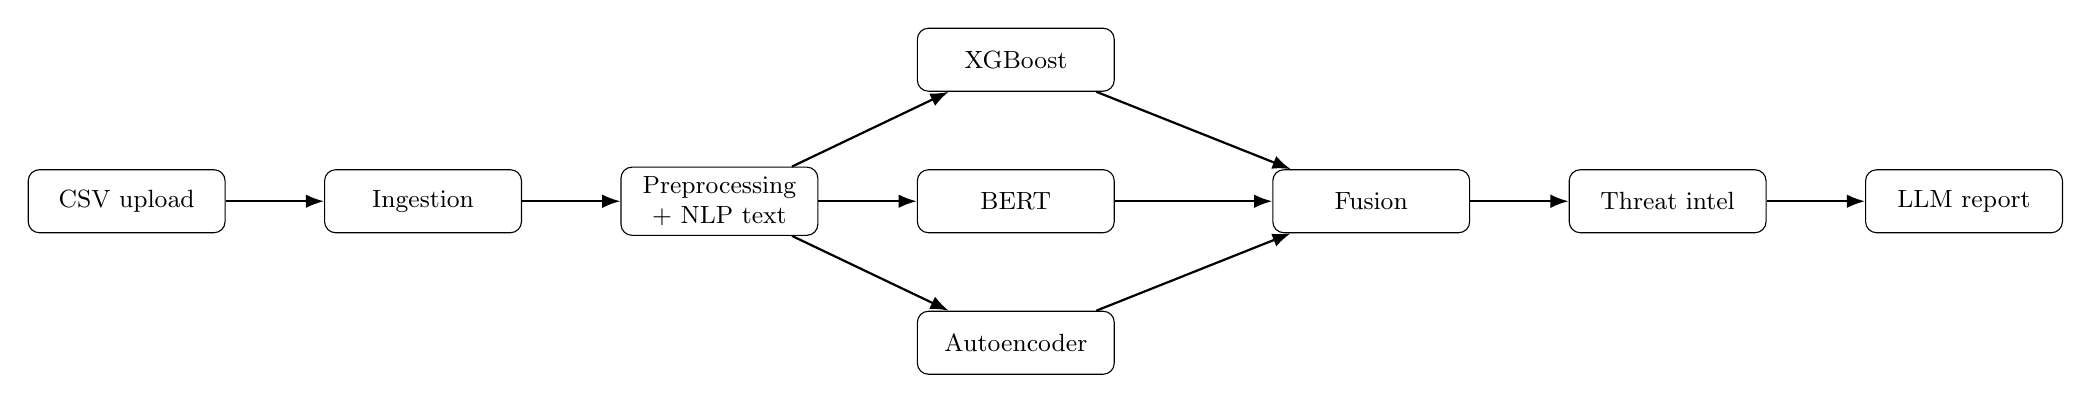
\begin{tikzpicture}[
    node distance=0.95cm and 1.25cm,
    box/.style={draw, rounded corners, align=center, minimum width=2.5cm, minimum height=0.8cm, font=\small},
    arrow/.style={-Latex, thick}
]
    \node[box] (csv) {CSV upload};
    \node[box, right=of csv] (ingest) {Ingestion};
    \node[box, right=of ingest] (prep) {Preprocessing\\+ NLP text};
    \node[box, above right=of prep] (xgb) {XGBoost};
    \node[box, right=of prep] (bert) {BERT};
    \node[box, below right=of prep] (ae) {Autoencoder};
    \node[box, right=2.0cm of bert] (fusion) {Fusion};
    \node[box, right=of fusion] (mcp) {Threat intel};
    \node[box, right=of mcp] (llm) {LLM report};

    \draw[arrow] (csv) -- (ingest);
    \draw[arrow] (ingest) -- (prep);
    \draw[arrow] (prep) -- (xgb);
    \draw[arrow] (prep) -- (bert);
    \draw[arrow] (prep) -- (ae);
    \draw[arrow] (xgb) -- (fusion);
    \draw[arrow] (bert) -- (fusion);
    \draw[arrow] (ae) -- (fusion);
    \draw[arrow] (fusion) -- (mcp);
    \draw[arrow] (mcp) -- (llm);
\end{tikzpicture}
}
\caption{Runtime architecture of the Cyber AI Agent backend.}
\label{fig:architecture}
\end{figure}

\subsection{Backend Implementation}

The backend is implemented in Python using FastAPI. The main application is defined in \texttt{backend/app/main.py}; the pipeline orchestration is in \texttt{backend/app/pipeline.py}. Each AI step is isolated in \texttt{backend/app/layers/}, which makes the system easier to test and debug.

\begin{table}[H]
\centering
\caption{Backend Components and Responsibilities}
\label{tab:backend_components}
\small
\begin{tabularx}{\linewidth}{l X}
\toprule
File / module & Responsibility \\
\midrule
\texttt{main.py} & Creates the FastAPI application, enables CORS, loads environment variables, and registers API routers. \\
\texttt{pipeline.py} & Loads singleton layer objects, executes all eight layers, serializes debug outputs, and returns final results. \\
\texttt{ingestion.py} & Parses uploaded CSV content and validates the 18 required features. \\
\texttt{preprocessing.py} & Reindexes features, cleans invalid values, applies the saved scaler, and generates text descriptions. \\
\texttt{xgboost\_model.py} & Loads \texttt{xgboost\_model.pkl} and returns labels, attack names, and probabilities. \\
\texttt{bert\_model.py} & Loads the local BERT classifier and tokenizes generated texts for inference. \\
\texttt{autoencoder\_model.py} & Loads \texttt{autoencoder.keras} and \texttt{autoencoder\_threshold.json}; returns reconstruction error and anomaly flags. \\
\texttt{fusion.py} & Combines model outputs, resolves labels, calculates fused risk score, and creates the threat list. \\
\texttt{mcp\_tools.py} & Adds local IP reputation and CVE mapping to detected threats. \\
\texttt{llm\_explainer.py} & Produces structured JSON explanations using Groq or a deterministic mock fallback. \\
\bottomrule
\end{tabularx}
\end{table}

\subsection{API and Frontend Product}

The product includes a React + Vite frontend. The demo workflow begins on the upload page, where the user selects a CSV file. The frontend sends the file to \texttt{/api/upload-logs}, then triggers \texttt{/api/predict?debug=true}. After prediction, the dashboard displays summary statistics, threat severity distribution, attack type distribution, per-model breakdown, LLM reports, and layer-by-layer debug telemetry.

\begin{table}[H]
\centering
\caption{Main API Endpoints}
\label{tab:api}
\begin{tabularx}{\linewidth}{l l X}
\toprule
Method & Endpoint & Purpose \\
\midrule
GET & \texttt{/} & Health check and documentation pointer. \\
POST & \texttt{/api/upload-logs} & Upload a CSV log file. \\
POST & \texttt{/api/predict} & Run the full pipeline on an uploaded file. \\
GET & \texttt{/api/dashboard} & Return latest summary, threat counts, and model breakdown. \\
GET & \texttt{/api/reports} & Return enriched LLM threat reports. \\
GET & \texttt{/api/debug/runs} & List saved debug run IDs. \\
GET & \texttt{/api/debug/run/\{run\_id\}} & Load a specific debug trace. \\
GET & \texttt{/api/debug/latest} & Load the latest debug trace. \\
\bottomrule
\end{tabularx}
\end{table}

\subsection{Reproducibility}

The repository includes \texttt{backend/requirements.txt} for Python dependencies, \texttt{frontend/package.json} for the React frontend, setup instructions in the README and \texttt{SETUP.md}, and a \texttt{backend/.env.example} file for optional LLM configuration. Runtime model artifacts are loaded from \texttt{backend/trained\_models/}. The backend also writes JSON debug traces to \texttt{backend/debug\_logs/}, allowing intermediate outputs to be inspected after each run.

% ------------------------------------------------------------
\section{Experimental Setup and Results}

\subsection{Experimental Setup}

The dataset was split into training, validation, and test sets during preprocessing. XGBoost and BERT were evaluated as multiclass classifiers. The autoencoder was trained on benign traffic and evaluated as an anomaly detector using reconstruction error. The ensemble notebook then loaded all saved artifacts and compared individual and fused model behavior over the test split.

Metrics used:

\begin{itemize}[leftmargin=1.2cm]
    \item \textbf{Accuracy}: proportion of all correctly classified records.
    \item \textbf{Precision}: proportion of predicted attacks that are correct.
    \item \textbf{Recall}: proportion of actual attacks detected.
    \item \textbf{F1-score}: harmonic mean of precision and recall.
    \item \textbf{False positive rate}: benign records incorrectly flagged by the anomaly detector.
    \item \textbf{ROC-AUC}: separability measure for XGBoost probability outputs.
\end{itemize}

\subsection{Individual Model Results}

Table~\ref{tab:individual_results} reports the saved metrics from the individual model artifact files. These are the strongest direct indicators of each model's standalone performance.

\begin{table}[H]
\centering
\caption{Saved Individual Model Metrics}
\label{tab:individual_results}
\small
\begin{tabular}{l c c c c c}
\toprule
Model & Test samples & Accuracy & Precision & Recall & F1-score \\
\midrule
XGBoost & 241,522 & 0.9974 & 0.9973 & 0.9974 & 0.9969 \\
BERT & 91,484 & 0.9513 & 0.9424 & 0.9513 & 0.9465 \\
Autoencoder & 241,522 & 0.8853 & 0.7074 & 0.5726 & 0.6329 \\
\bottomrule
\end{tabular}
\end{table}

XGBoost produced the best standalone supervised result. This is expected because the dataset consists mainly of structured flow features, which are well suited to gradient-boosted decision trees. BERT also performed strongly, showing that the generated text representation preserved useful traffic behavior. The autoencoder had lower F1-score, but it serves a different purpose: identifying unusual behavior through reconstruction error rather than assigning an exact attack class.

\subsection{Autoencoder Threshold}

The saved autoencoder threshold is 0.0051889612, selected as the 95th percentile threshold. The validation F1-score at this threshold is 0.6302, and the test false positive rate is 0.0494. This supports its role as a supplementary anomaly detector rather than the only decision engine.

\subsection{Fusion and Ablation Results}

The ensemble experiment in \texttt{05\_ensemble.ipynb} saved the results in Table~\ref{tab:ensemble_results}. This notebook performs a separate combined inference run, so its individual model comparison values can differ from the standalone notebook files due to evaluation sample size and pipeline context.

\begin{table}[H]
\centering
\caption{Saved Ensemble Experiment Metrics}
\label{tab:ensemble_results}
\small
\begin{tabular}{l c c}
\toprule
Component & Accuracy & F1-score \\
\midrule
XGBoost in ensemble run & 0.9969 & 0.9964 \\
BERT in ensemble run & 0.8018 & 0.7364 \\
Autoencoder in ensemble run & -- & 0.6646 \\
Fusion ensemble & 0.9750 & 0.9713 \\
\bottomrule
\end{tabular}
\end{table}

The fusion result improves substantially over the weaker BERT and autoencoder signals in the ensemble experiment, but it does not exceed XGBoost. This is an important finding: multi-model fusion improves transparency and provides complementary evidence, but the current saved metrics show that XGBoost should be treated as the most reliable classifier for a production design.

\subsection{Training Cost}

\begin{table}[H]
\centering
\caption{Saved Training Times}
\label{tab:training_time}
\begin{tabular}{l c c}
\toprule
Model & Training time (seconds) & Approximate time \\
\midrule
XGBoost & 1788.15 & 29.8 minutes \\
BERT & 12968.83 & 3.6 hours \\
Autoencoder & 7427.44 & 2.1 hours \\
\bottomrule
\end{tabular}
\end{table}

BERT and the autoencoder require significantly more training time than XGBoost. This supports the practical decision to use XGBoost as the most important runtime classifier and to use the other models for complementary analysis and explanation.

% ------------------------------------------------------------
\section{Evaluation and Performance Analysis}

\subsection{Quantitative Evaluation}

From the saved metrics, XGBoost achieved the best balance of accuracy, recall, and F1-score. Its ROC-AUC value of 0.9920 further indicates strong probability separation. BERT's standalone metrics are also strong, but its ensemble-run metrics were weaker, suggesting that text-generation consistency, evaluation sample differences, or artifact alignment must be controlled carefully in future experiments. The autoencoder had a moderate F1-score but a low false positive rate of approximately 4.94\%, which is useful for prioritizing suspicious behavior.

\subsection{Qualitative Evaluation}

The qualitative strength of the system is interpretability. The dashboard does not only show a final label; it exposes XGBoost output, BERT output, autoencoder anomaly score, fused risk, severity, static threat-intelligence context, and a natural-language explanation. The debug page also allows layer-by-layer inspection, which is useful for identifying mismatches between training artifacts and runtime behavior.

\subsection{Comparison With Baselines}

A single XGBoost model is the strongest performance baseline in this project. The final system adds value beyond this baseline by providing:

\begin{itemize}[leftmargin=1.2cm]
    \item an independent transformer perspective from textual traffic descriptions;
    \item unsupervised anomaly evidence from reconstruction error;
    \item static IP/CVE enrichment for analyst context;
    \item LLM or mock explanations for readable reports;
    \item frontend visualization and debug traceability.
\end{itemize}

Therefore, the project should not be judged only as a marginal F1-score optimization. It is a full AI product that combines detection, explanation, and demonstration usability.

% ------------------------------------------------------------
\section{Discussion}
\label{sec:discussion}

\subsection{Strengths}

The project is strong in four areas. First, it implements more than the minimum number of required Advanced AI techniques. Second, it is end-to-end: the system includes training notebooks, saved artifacts, an API, and a frontend. Third, the pipeline is modular, so each layer can be tested or replaced. Fourth, the dashboard and debug route make model behavior visible, which improves trust and supports demonstration.

\subsection{Limitations}

The current backend fusion logic allows any of the three detectors to mark a record as a threat. This improves sensitivity but can also increase inconsistency when one model is overconfident or misaligned. The saved ensemble metrics also show that fusion does not outperform XGBoost. Therefore, the current system is best described as an explainable multi-model research prototype rather than a fully calibrated production SOC detector.

The static threat-intelligence layer is intentionally limited. It uses a small local blacklist and CVE map, not a live reputation service. This is appropriate for coursework demonstration but should not be described as real-time threat intelligence.

The LLM layer depends on a Groq API key for live explanations. When no key is configured, the system uses mock explanations. This keeps the product demonstrable, but live LLM behavior should be evaluated separately for reliability and factual safety.

\subsection{Recommended Production Refinement}

The saved results support a future XGBoost-centric production design. In that design, XGBoost would be the only final attack classifier, the autoencoder would only raise or lower risk based on anomaly score, and the language model would be used only after the decision for explanation. This avoids conflicting votes and prevents BERT or anomaly-only outputs from overriding the strongest classifier.

A production decision rule could be:

\begin{lstlisting}[language=Python, caption={Recommended future production decision rule}]
pred = xgb_model.predict(X)
is_anomaly = autoencoder_score(X) > threshold

if pred != "BENIGN":
    label = pred
    severity = "HIGH" if is_anomaly else "MEDIUM"
else:
    label = "BENIGN"
    severity = "LOW" if is_anomaly else "VERY_LOW"
\end{lstlisting}

This refinement should be described as future work unless the backend code is changed to match it.

% ------------------------------------------------------------
\section{Conclusion and Future Work}

Cyber AI Agent successfully demonstrates a complete Advanced Artificial Intelligence project in the cybersecurity domain. It combines NLP, transformer transfer learning, unsupervised autoencoder anomaly detection, ensemble fusion, prompt-engineered explanation, a FastAPI backend, and a React dashboard. The project therefore addresses all major assignment requirements: real-world relevance, multiple AI techniques, model implementation, evaluation, report quality, and working demo functionality.

The evaluation shows that XGBoost is the strongest classifier for the structured flow dataset, while BERT and the autoencoder add complementary interpretability and anomaly evidence. The final product is suitable for a coursework demonstration and provides a clear foundation for future hardening.

Future work should focus on:

\begin{enumerate}[leftmargin=1.2cm]
    \item implementing the XGBoost-centric production decision rule;
    \item calibrating severity thresholds on a validation set;
    \item replacing static IP/CVE lookup tables with live threat-intelligence APIs;
    \item adding model and data versioning for reproducibility;
    \item expanding frontend reporting to export PDF/CSV incident summaries;
    \item adding continuous integration so backend tests and frontend builds run automatically.
\end{enumerate}

% ------------------------------------------------------------
\section{References}

\begin{thebibliography}{9}

\bibitem{bert}
Devlin, J., Chang, M.-W., Lee, K., \& Toutanova, K. (2019). BERT: Pre-training of deep bidirectional transformers for language understanding. \textit{Proceedings of the 2019 Conference of the North American Chapter of the Association for Computational Linguistics: Human Language Technologies}, 4171--4186.

\bibitem{vaswani}
Vaswani, A., Shazeer, N., Parmar, N., Uszkoreit, J., Jones, L., Gomez, A. N., Kaiser, L., \& Polosukhin, I. (2017). Attention is all you need. \textit{Advances in Neural Information Processing Systems}, 30.

\bibitem{xgboost}
Chen, T., \& Guestrin, C. (2016). XGBoost: A scalable tree boosting system. In \textit{Proceedings of the 22nd ACM SIGKDD International Conference on Knowledge Discovery and Data Mining} (pp. 785--794).

\bibitem{sklearn}
Pedregosa, F., Varoquaux, G., Gramfort, A., Michel, V., Thirion, B., Grisel, O., Blondel, M., Prettenhofer, P., Weiss, R., Dubourg, V., Vanderplas, J., Passos, A., Cournapeau, D., Brucher, M., Perrot, M., \& Duchesnay, E. (2011). Scikit-learn: Machine learning in Python. \textit{Journal of Machine Learning Research, 12}, 2825--2830.

\bibitem{cicids}
Sharafaldin, I., Lashkari, A. H., \& Ghorbani, A. A. (2018). Toward generating a new intrusion detection dataset and intrusion traffic characterization. \textit{Proceedings of the 4th International Conference on Information Systems Security and Privacy}, 108--116.

\bibitem{rumelhart}
Rumelhart, D. E., Hinton, G. E., \& Williams, R. J. (1986). Learning representations by back-propagating errors. \textit{Nature, 323}(6088), 533--536.

\bibitem{fastapi}
Ramirez, S. (2024). \textit{FastAPI documentation}. https://fastapi.tiangolo.com/

\end{thebibliography}

% ------------------------------------------------------------
\appendix
\section{Appendices}

\subsection{Core Project Structure}

\begin{lstlisting}[caption={Core project structure}]
cyber-ai-agent/
|-- backend/
|   |-- app/
|   |   |-- main.py
|   |   |-- pipeline.py
|   |   |-- layers/
|   |   |-- routes/
|   |   |-- models/
|   |   +-- utils/
|   |-- notebooks/
|   |-- tests/
|   |-- trained_models/
|   |-- requirements.txt
|   +-- init_models.py
|-- frontend/
|   |-- src/
|   |-- package.json
|   +-- vite.config.js
|-- reports/
|-- README.md
+-- SETUP.md
\end{lstlisting}

\subsection{Runtime Commands}

\begin{lstlisting}[caption={Backend and frontend demo commands}]
cd backend
.\venv\Scripts\Activate.ps1
uvicorn app.main:app --reload --port 8000

cd frontend
npm install
npm run dev
\end{lstlisting}

\subsection{Team Contribution Breakdown}

\begin{table}[H]
\centering
\caption{Team Contribution Template}
\begin{tabularx}{\linewidth}{l X}
\toprule
Member & Contribution \\
\midrule
Student Name 1 & Data preprocessing, XGBoost training, metric analysis. \\
Student Name 2 & BERT training, autoencoder training, notebook documentation. \\
Student Name 3 & FastAPI backend, React dashboard, report and presentation preparation. \\
\bottomrule
\end{tabularx}
\end{table}

\subsection{Submission Checklist}

\begin{itemize}[leftmargin=1.2cm]
    \item Final report uses required sections, 12 pt font, 1.5 spacing, 1 inch margins, page numbers, and references.
    \item README and SETUP guide describe dependencies and reproducible execution.
    \item Training notebooks contain markdown explanations and save artifacts.
    \item Backend can run on port 8000 and frontend on port 3000.
    \item Video presentation should cover problem, approach, results, and live dashboard demo within five minutes.
\end{itemize}

\end{document}
